\begin{center}
    \begin{tabular}{c|c}
        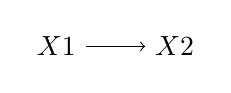
\begin{tikzpicture}
            \node (v0) at (0,0) {$X1$};
            \node (v1) at (1.5,0) {$X2$};
            \draw [->] (v0) edge (v1);
        \end{tikzpicture}\\
         &  
        \begin{tikzpicture}
            \draw (0,0) node[circleobject] (1) {$V_1$};
            \draw (1.5,0) node[circleobject] (2) {$V_2$};
            \draw (3,0) node[circleobject] (3) {$V_3$};
            \draw (4.5,0) node[circleobject] (4) {$V_4$};
            \draw (6,0) node[circleobject] (5) {$V_5$};
            \draw[-latex]  (1) edge (2);
            \draw[-latex,bend right]  (1) edge (3);
            \draw[-latex,bend right]  (3) edge (5);
            \draw[-latex,bend left]  (2) edge (4);
        \end{tikzpicture}
        \captionof{figure}{Topological order of graph}
        \label{fig:topological order}
    \end{tabular}
\end{center}